\documentclass[
	10pt,								% globale Schriftgröße
	parskip=half-,						% setzt Absatzabstand hoch
	paper=a4,							% Format
	english,
	appendixprefix=true					% lädt Sprachpakete
	]{scrartcl}							% Dokumentenklasse
%\linespread{1.2} % Increase line spacing
% //////////////////// Pakete laden ////////////////////
\usepackage{amsmath}			% MUSS vor fontspec geladen werden
\usepackage{mathtools}			% modifiziert amsmath
\usepackage{amssymb}			% mathematische symbole, für \ceckmarks
\usepackage{amsthm}				% für proof
\usepackage{mathrsfs}			% für \mathscr
\usepackage{latexsym}
\usepackage{marvosym}				% für Lightning

%%% to allow custom headings
\usepackage{titlesec}
% to change titles font family
\usepackage{titling}

\usepackage{fontspec} 			% funktioniert nur mit den neueren Compilern z.B. XeLaTeX
\usepackage{microtype}			% für bessere Worttrennung
\usepackage[ngerman]{babel} 	% Spracheinstellung
\usepackage{lmodern}			% verändert verwendete Schriftart, damit sie weniger pixelig ist

\usepackage{verbatim}
\usepackage{listings}			% Für Quellcode

\usepackage{graphicx}
\usepackage{subcaption}
\usepackage{tabularx}			% für Tabellen mit gleicher Spaltenbreite und automatischen Umbrüchen
\usepackage{fullpage}
\usepackage{multirow}			% für multirow in tabulars
\usepackage{rotate}
\usepackage[cmyk,table]{xcolor} % um Farben zu benutzen, kann mehr als das Paket color
\usepackage[					% Verlinkungen
	colorlinks,					% farbige Schrift, statt farbiger Rahmen
	linktocpage,				% verlinkt im Abb.Verzeichnis Seitenzahl statt Bildunterschrift
	linkcolor=blue,				% setzt Farbe der Links auf blau
	urlcolor=blue	
	]{hyperref}					% nur für digitale Anwendungen, url = "http://www.example.com"
\usepackage{url}				% für Webadressen wie e-mail usw.: "\url{http://www.example.com}"
\urlstyle{sf}

\usepackage{enumerate}			% für versch. Aufzählungezeichen wie z.B. a)
\usepackage{xspace}				% folgt ein Leerzeichen nach einem \Befehl, wird es nicht verschluckt.
\usepackage{cancel}				% für das Durchstreichen u.a. in Matheformeln mit \cancel
\usepackage{float}              % zum Forcieren der Position von figure-Umgebungen

% Change font of document
\setsansfont{Source Sans Pro}
\setmainfont{Source Sans Pro}
% font declaration and title settings
\newfontfamily\headingfont[]{Source Sans Pro Light}
\titleformat{\chapter}[display]
  {\huge\headingfont}{\chaptertitlename\ \thechapter}{26pt}{\Huge}
\titleformat*{\section}{\LARGE\headingfont}
\titleformat*{\subsection}{\Large\headingfont}
\renewcommand{\maketitlehooka}{\headingfont}

\newfontfamily\ttfamily[]{Roboto Mono}
% zum Zeichnen (u.a. von Graphen)
\usepackage{fp}
\usepackage{tikz}
\usetikzlibrary{tikzmark}			% für \tikzmark{toRemember}
\usetikzlibrary{positioning}	% verbesserte Positionierung der Knoten
\usetikzlibrary{automata}		% für Automaten (GTI)
\usetikzlibrary{arrows}
\usetikzlibrary{shapes}
\usetikzlibrary{decorations.pathmorphing}
\usetikzlibrary{decorations.pathreplacing}
\usetikzlibrary{decorations.shapes}
\usetikzlibrary{decorations.text}

% //////////////////// Syntaxhighlighting ////////////////////
\lstloadlanguages{Python, Haskell, [LaTeX]TeX, Java}
\lstset{
   basicstyle=\footnotesize\ttfamily,	% \scriptsize the size of the fonts that are used for the code
   backgroundcolor = \color{bgcolour},	% legt Farbe der Box fest
   breakatwhitespace=false,	% sets if automatic breaks should only happen at whitespace
   breaklines=true,			% sets automatic line breaking
   captionpos=t,				% sets the caption-position to bottom, t for top
   commentstyle=\color{codeblue}\ttfamily,% comment style
   frame=single,				% adds a frame around the code
   keepspaces=true,			% keeps spaces in text, useful for keeping indentation
							% of code (possibly needs columns=flexible)
   keywordstyle=\bfseries\ttfamily\color{codepurple},% keyword style
   numbers=left,				% where to put the line-numbers;
   							% possible values are (none, left, right)
   numberstyle=\tiny\color{codegreen},	% the style that is used for the line-numbers
   numbersep=5pt,			% how far the line-numbers are from the code
   stepnumber=1,				% nummeriert nur jede i-te Zeile
   showspaces=false,			% show spaces everywhere adding particular underscores;
							% it overrides 'showstringspaces'
   showstringspaces=false,	% underline spaces within strings only
   showtabs=false,			% show tabs within strings adding particular underscores
   flexiblecolumns=false,
   tabsize=1,				% the step between two line-numbers. If 1: each line will be numbered
   stringstyle=\color{orange}\ttfamily,	% string literal style
   numberblanklines=false,				% leere Zeilen werden nicht mitnummeriert
   xleftmargin=1.2em,					% Abstand zum linken Layoutrand
   xrightmargin=0.4em,					% Abstand zum rechten Layoutrand
   aboveskip=2ex, 
}

\lstdefinestyle{py}{
   language=Python,
}
\lstdefinestyle{hs}{
   language=Haskell,
}
\lstdefinestyle{tex}{
	language=[LaTeX]TeX,
	escapeinside={\%*}{*)},     % if you want to add LaTeX within your code
	texcsstyle=*\bfseries\color{blue},% hervorhebung der tex-Schlüsselwörter
	morekeywords={*,$,\{,\},\[,\],lstinputlisting,includegraphics,
	rowcolor,columncolor,listoffigures,lstlistoflistings,
	subsection,subsubsection,textcolor,tableofcontents,colorbox,
	fcolorbox,definecolor,cellcolor,url,linktocpage,subtitle,
	subject,maketitle,usetikzlibrary,node,path,addbibresource,
	printbibliography},% if you want to add more keywords to the set
     numbers=none,
     numbersep=0pt,
     xleftmargin=0.4em,
}

\lstdefinestyle{java}{
	language=Java,
	extendedchars=true,		% lets you use non-ASCII characters;
   						% for 8-bits encodings only, does not work with UTF-8
}

\lstdefinelanguage[x64]{Assembler}     % add a "x64" dialect of Assembler
   [x86masm]{Assembler} % based on the "x86masm" dialect
   % with these extra keywords:
   {morekeywords={CDQE,CQO,CMPSQ,CMPXCHG16B,JRCXZ,LODSQ,MOVSXD, %
                  POPFQ,PUSHFQ,SCASQ,STOSQ,IRETQ,RDTSCP,SWAPGS, %
                  rax,rdx,rcx,rbx,rsi,rdi,rsp,rbp, %
                  r8,r8d,r8w,r8b,r9,r9d,r9w,r9b}
}					% for 8-bits encodings only, does not work with UTF-8

\lstdefinestyle{c}{
	language=c,
	extendedchars=true,		% for 8-bits encodings only, does not work with UTF-8
}

% //////////////////// eigene Kommandos ////////////////////
\newcommand\FU{Freie Universität Berlin\xspace}% benötigt package xspace
\newcommand\gdw{g.\,d.\,w.\xspace}
\newcommand\oBdA{o.\,B.\,d.\,A.\xspace}
\newcommand{\Eu}{\texteuro}
\newcommand\N{\mathbb{N}\xspace}
\newcommand\Q{\mathbb{Q}\xspace}
\newcommand\R{\mathbb{R}\xspace}
\newcommand\Z{\mathbb{Z}\xspace}
\newcommand\ohneNull{\ensuremath{\backslash\lbrace 0\rbrace}}% \{0}
\let\dhALT\dh	% Schreibt Befehl \dh in \dhALT um
\renewcommand\dh{d.\,h.\xspace}	%renew überschreibt command \dh
\newcommand\Bolt{\;\text{\LARGE\raisebox{-0.3em}{\Lightning}\normalsize}\xspace}% Blitz
\newcommand\zz{\ensuremath{\raisebox{+0.25ex}{Z}% zu zeigen
			\kern-0.4em\raisebox{-0.25ex}{Z}%
			\;\xspace}}
\newcommand{\from}{\ensuremath{\colon}}
\newcommand{\floor}[1]{\lfloor{#1}\rfloor}
\newcommand{\ceil}[1]{\lceil{#1}\rceil}
 \renewcommand{\L}{\ensuremath{\mathcal{L}}\xspace}
 \renewcommand{\P}{\ensuremath{\mathcal{P}}\xspace}
 \newcommand{\NL}{\ensuremath{\mathcal{N}\kern-0.2em\mathcal{L}}\xspace}
 \newcommand{\NP}{\ensuremath{\mathcal{NP}}\xspace}

% //////////////////// Mathefunktionen ////////////////////
\DeclareMathOperator{\Landau}{\mathcal{O}}
\DeclareMathOperator{\True}{True}
\DeclareMathOperator{\False}{False}

% //////////////////// eigene Theoreme ////////////////////
\newtheorem{theorem}{Satz}
\newtheorem{corollary}[theorem]{Folgerung}
\newtheorem{lemma}[theorem]{Lemma}
\newtheorem{observation}[theorem]{Beobachtung}
\newtheorem{definition}[theorem]{Definition}
\newtheorem{Literatur}[theorem]{Literatur}
% konfiguriert proof
\makeatletter
\newenvironment{Proof}[1][\proofname]{\par
  \pushQED{\qed}%
  \normalfont \topsep6\p@\@plus6\p@\relax
  \trivlist
  \item[\hskip\labelsep
%         \itshape
        \bfseries
    #1\@addpunct{.}]\ignorespaces
}{%
  \popQED\endtrivlist\@endpefalse
}
\makeatother

% //////////////////// eigene Farben ////////////////////
\let\definecolor=\xdefinecolor
\definecolor{FUgreen}{RGB}{153,204,0}
\definecolor{FUblue}{RGB}{0,51,102}

\definecolor{middlegray}{rgb}{0.5,0.5,0.5}
\definecolor{lightgray}{rgb}{0.8,0.8,0.8}
\definecolor{orange}{rgb}{0.8,0.3,0.3}
\definecolor{azur}{rgb}{0,0.7,1}
\definecolor{yac}{rgb}{0.6,0.6,0.1}
\definecolor{Pink}{rgb}{1,0,0.6}

\definecolor{bgcolour}{rgb}{0.97,0.97,0.97}
\definecolor{codegreen}{rgb}{0,0.6,0}
\definecolor{codegray}{rgb}{0.35,0.35,0.35}
\definecolor{codepurple}{rgb}{0.58,0,0.82}
\definecolor{codeblue}{rgb}{0.4,0.5,1}

% //////////////////// eigene Settings ////////////////////

\textheight = 230mm		% Höhe des Satzspiegels / Layouts
\footskip = 10ex			% Abstand zw. Fußzeile und Grundlinie letzter Textzeile
\parindent 0pt			% verhindert Einrückung der 1. Zeile eines Absatzes
\setkomafont{sectioning}{\rmfamily\bfseries}% setzt Ü-Schriften in Serifen, {disposition}

\usepackage{booktabs}
\usepackage[babel, german=quotes]{csquotes} % einfache Handhabung von quotations
\usepackage[backend=biber]{biblatex} %biblatex mit biber laden
\ExecuteBibliographyOptions{
sorting=nyt, %Sortierung Autor, Titel, Jahr
bibwarn=true, %Probleme mit den Daten, die Backend betreffen anzeigen
isbn=false, %keine isbn anzeigen
url=false %keine url anzeigen
}											% bindet Header ein

\renewcommand{\arraystretch}{1.2} % more whitespace in tables
\usepackage{array} % Being able to format columns of tables
\addbibresource{lit.bib} %Bibliographiedateien laden

\begin{document}
 
\title{Final Course Assignment \\ }%replace X with the appropriate number
\author{Mark Niehues, Stefaan Hessmann \\ %replace with your name
Mathematical Aspects in Machine Learning} %if necessary, replace with your course title

\maketitle
 
\section{Introduction}
In the past course we dealt with the broad mathematical foundations of machine learning. To get an idea of what the consequences of those mathematical theorems and approaches are and to get in touch with the standard Python tools, we have evaluated an comparatively easy data science example found on \url{kaggle.com}. Since this was our first machine learning project, we decided to deal with an rather simple problem. The example dataset \cite{Kaggle2017} consists of the historic passenger records of the disastrous Titanic maiden voyage in 1912. The goal in this Challenge was to predict if a passenger survived the accident based on informations like for example age, sex and payed ticket fare. Therefore it is in terms of machine learning a \textit{classification problem} with two classes: survived and not survived.

Inspired by sample solutions from the website, we first took a deeper look on the dataset and tried to select the most significant influences by reviewing the statistical properties of the dataset. In the following we implemented an naive Sequential Minimal Optimization (SMO) algorithm and ran a few tests with them in order to finally compare the results with other machine learning algorithms.

\section{Applying Machine Learning Methods on the Titanic Disaster}
\subsection{Dataset}
The given dataset consists of a CSV-file containing data of 891 passengers. The dataset contains an ID for every passenger, a label if the passenger has survived the disaster and the features that are described in table \ref{tab:features}. It can be noticed that some of the features are incomplete.

\begin{table}
\caption{Features and their amount of missing data.}
\begin{tabular}{>{\bfseries}l l l}
PassengerId & Unique ID for every passenger & 0.0 \%\\
Survived & Survived (1) or died (0) & 0.0 \% \\
Pclass & Passenger's class & 0.0 \% \\
Name & Passenger's name & 0.0 \% \\
Sex & Passenger's sex & 0.0 \% \\
Age & Passenger's age & \textbf{19.87 \%} \\
SibSp & Number of siblings/spouses aboard & 0.0 \% \\
Parch & Number of parents/children aboard & 0.0 \% \\
Ticket & Ticket number & 0.0 \% \\
Fare & Ticket-price & 0.0 \% \\
Cabin & Number of the passenger's cabin & \textbf{77.10 \%} \\
Embarked & Port of embarkation & \textbf{0.22 \%} \\
\end{tabular}
\centering
\label{tab:features}
\end{table}

After loading the dataset, it is necessary to process the data for our learning machine. Therefore the different features will be investigated to select meaningful features and the missing data needs to be handled.

\subsection{Feature: Sex}
The sex-feature divides the passengers into the categories 'female' and 'male'. Figure \ref{fig:sexfeat} shows the probability of survival for male and female passengers. It is obvious that females had a much higher probability to survive than the male passengers. 'Sex' seems to be a useful feature for the learning machine.
 \begin{figure}
 	\centering
    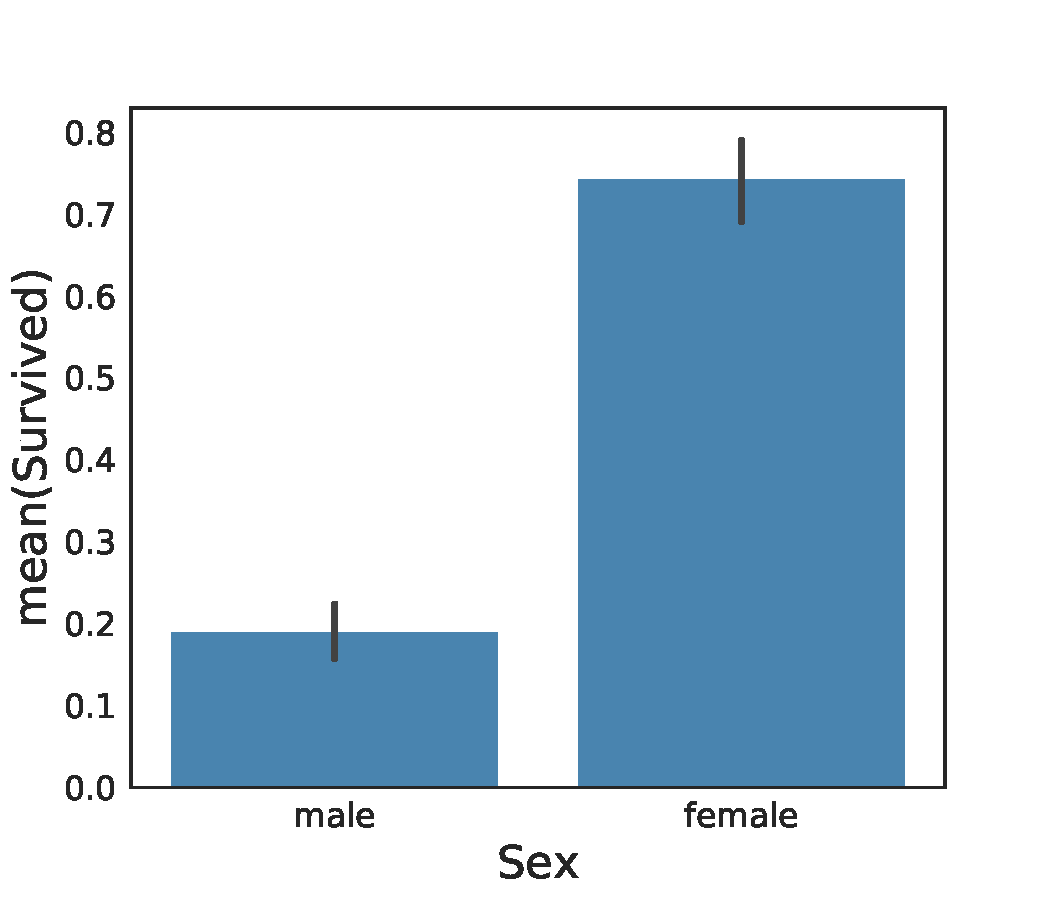
\includegraphics[width=0.5\textwidth]{media_saved/sex_survived}
  \caption{Survival probability depending on the passenger's sex.}
  \label{fig:sexfeat}
 \end{figure}

\subsection{Feature: Age}
The impact of a passengers' age on their probability to survive categorized by their sex is pointed out 

\section{Implementation of an easy SMO Algorithm}
To get a better understanding of what a Support Vector Machine does, we decided to implement one on our own using several publications. Most of them were based on the important paper of Platt \cite{platt} where he introduced a new approach for the calculation of the Support Vectors that improves the performance a lot. This algorithm is called Sequential Minimal Optimization. Performance was not the highest priority for us but instead understandability and the costs of implementation. Therefore we implemented a less complex version of the algorithm presented in Platt's paper.

\section*{Appendix}
\appendix
\section{Pseudo Code of the SMO algorithm}
\begin{figure}[!h]
  \centering
    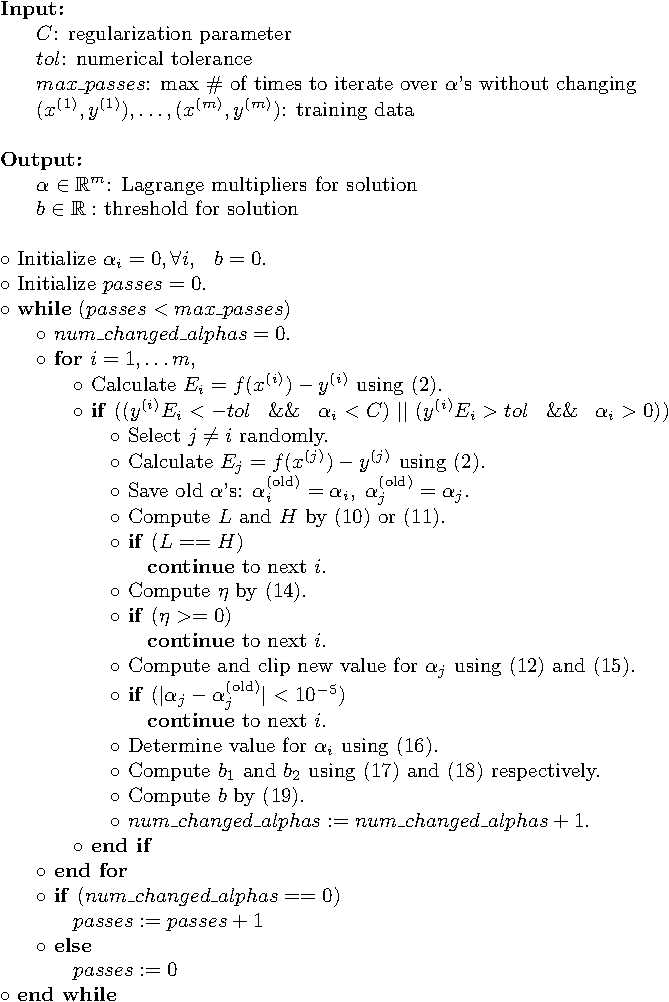
\includegraphics[width=0.8\textwidth]{media_saved/pseudo_code}
  \label{fig:gull}
\end{figure}

\section{Code}
\lstinputlisting[
	style=py,									% Style
	firstnumber={0},										% Start der Nummerierung
	firstline={15}											% 1. Codezeile
]											% letzte Codezeile
{./own_svm/kernels.py}

\printbibliography %hier Bibliographie ausgeben lassen
\end{document}        
